%!TEX root = ../../novoIndex.tex
A fim de adequar melhor o conjunto de dados para os modelos de CNNs utilizados, realizou-se uma limpeza e pré-processamento dos meta-dados e das imagens da base IMDb, que se iniciou com o cálculo do atributo alvo, a idade, a partir dos atributos originais fornecidos. A idade foi aferida através da data de nascimento da celebridade e do ano em que a fotografia em questão foi capturada.

Uma análise do conjunto de dados revelou a presença de itens com idade e gênero apresentando valores nulos, inválidos ou negativos, que foram descartados. Observou-se também a presença de múltiplos exemplos referentes à mesma pessoa com a mesma idade. Houve a remoção de tais exemplos, a fim de evitar que a apresentação de um mesmo rosto com a mesma idade provocasse \emph{overfitting} nos modelos. Exemplos atípicos, possivelmente resultados de rotulação incorreta, como idade maior que $100$ anos ou não compatível com os dados da celebridade referida nos meta-dados também foram descartados. Os atributos de pontuação de rostos foram úteis para identificar e remover exemplos em que não havia nenhum rosto identificado, ou em que havia mais de uma face na imagem. Este descarte foi realizado com o objetivo de eliminar rotulações errôneas, como a mostrada na Tabela \ref{tab:dois_deniro_errado}.

A última etapa consistiu na padronização das dimensões das imagens. Considerando a literatura, definiu-se o tamanho para $224 \times 224$ \emph{pixels} e o modo RGB como padrões. Por fim, após a padronização das imagens de entrada, o cálculo do atributo alvo idade, a adequação do caminho para as imagens em disco e a remoção de exemplos impróprios, seguiu-se o descarte dos outros meta-dados irrelevantes para a tarefa de estimação de idade de um indivíduo a partir de imagem. A data em que a foto foi tirada, nome, número de identificação, gênero, data de nascimento, localização do rosto da celebridade e pontuações de rostos nas imagens foram removidos.

Por fim, o conjunto de dados consolidado consiste de $47.950$ exemplos contendo imagens e idades de $14.607$ celebridades distintas, ocupando $1,2 GB$. O histograma de frequência da distribuição de idades de 0 a 100 anos presente nos exemplos da base de dados pode ser visualizado na Figura \ref{fig:hist}. Este total foi então dividido como proposto: conjunto de treinamento, contendo $70\%$ dos exemplos, ou seja, $33.565$ amostras; conjunto de validação, referente a $10\%$ dos dados, ou seja, $4.795$ itens; e, por fim, conjunto de testes, contendo os $20\%$ restantes, ou seja, $9.590$ exemplos.

\begin{figure}[!ht]
    \centering
     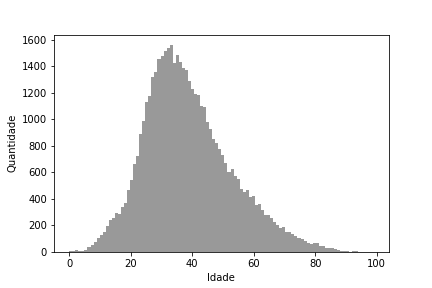
\includegraphics[width=0.7\textwidth]{img/idade_hist_clean}
     \caption{Histograma de frequência da idade do conjunto de dados utilizado.}
     \label{fig:hist}
\end{figure}
